\documentclass[twoside,twocolumn]{article}
\usepackage{blindtext}
\usepackage{graphicx}
\usepackage[sc]{mathpazo}
\usepackage[T1]{fontenc}
\linespread{1.05}
\usepackage{microtype}
\usepackage[english, spanish]{babel}
\usepackage[hmarginratio=1:1,top=32mm,columnsep=20pt]{geometry}
\usepackage[hang, small,labelfont=bf,up,textfont=it,up]{caption}
\usepackage{booktabs}
\usepackage{lettrine}
\usepackage{enumitem}
\setlist[itemize]{noitemsep}
\usepackage{abstract}
\renewcommand{\abstractnamefont}{\normalfont\bfseries} 
\renewcommand{\abstracttextfont}{\normalfont\small\itshape} 
\usepackage{titlesec}
\renewcommand\thesection{\Roman{section}} % 
\renewcommand\thesubsubsection{\roman{subsubsection}} 
\titleformat{\section}[block]{\large\scshape\centering}{\thesection.}{1em}{}
\titleformat{\subsubsection}[block]{\large}{\thesubsubsection.}{1em}{}
\usepackage{fancyhdr} 
\pagestyle{fancy} % All pages have headers and footers
\fancyhead{} % Blank out the default header
\fancyfoot{} % Blank out the default footer
\fancyhead[L]{MLOps} % Custom header text
\fancyhead[R]{Junio 2021} % Custom header text
\fancyfoot[RO,LE]{\thepage} % Custom footer text
\usepackage{titling}
\usepackage{hyperref}

%----------------------------------------------------------------------------------------
%	TILULOS
%----------------------------------------------------------------------------------------

\setlength{\droptitle}{-4\baselineskip}

\pretitle{\begin{center}\Huge\bfseries}
\posttitle{\end{center}} 
\title{MLOps}
\author{Jose Arias, Jose Gutierrez, Posi Vargas, Rodrigo Yanqui, Roby Zuñiga}
\date{\today} 
\renewcommand{\maketitlehookd}{
    \selectlanguage{spanish}
    \begin{abstract}
        \noindent A medida que las empresas profundizan su compromiso con el aprendizaje automático, están descubriendo no solo sus beneficios, sino también sus desafíos. Las encuestas definitivas no parecen estar disponibles, pero numerosos líderes de opinión han notado que muchos modelos de ML (algunos dicen que llegan al 70-80\%) nunca pasan de la etapa de prototipo a la producción.\\[0.1in]
        Una razón comúnmente citada para esta alta tasa de fallas es la dificultad de cerrar la brecha entre los científicos de datos que construyen y entrenan los modelos de inferencia y el equipo de TI que mantiene la infraestructura, así como los equipos de ingeniería de aprendizaje automático que desarrollan e implementan listos para producción. Aplicaciones de AA.\\[0.1in]
        Examinaremos más de cerca los desafíos que impiden que el aprendizaje automático alcance su potencial de cambio total y discutiremos cómo una disciplina relativamente nueva, las operaciones de aprendizaje automático o MLOps, es la clave para optimizar el ciclo de vida de las aplicaciones de aprendizaje automático.
    \end{abstract}
    \selectlanguage{english}
    \begin{abstract}
        \noindent As companies deepen their commitment to machine learning, they are discovering not only its benefits, but also its challenges. Definitive surveys do not appear to be available, but many opinion leaders have noted that many ML models (some reaching 70-80\%) never make it from prototype to production.\\[0.1in]
        One reason cited for this high failure rate is the difficulty of bridging the gap between the data scientists who build and train the inference models and the IT team that maintains the infrastructure, as well as the machine learning engineering teams that develop. and deployed ready for production. AA applications.\\[0.1in]
        We'll take a closer look at the challenges preventing machine learning from reaching its full potential for change and discuss how one relatively discipline, Machine Learning Operations, or MLOps, is the key to optimizing the lifecycle of machine learning applications.
    \end{abstract}
}

%----------------------------------------------------------------------------------------

\begin{document}

% Print the title
\maketitle

%----------------------------------------------------------------------------------------
%	INTRODUCCION
%----------------------------------------------------------------------------------------

\section{Introduccion}
\lettrine[nindent=0em,lines=3]{L}Los orígenes de MLOps se remontan a 2015 a partir de un artículo titulado "Deuda técnica oculta en sistemas de aprendizaje automático". Y desde entonces, el crecimiento ha sido particularmente fuerte. Tenga en cuenta que se espera que el mercado de soluciones MLOps alcance los \$4 mil millones para 2025..

%----------------------------------------------------------------------------------------
%	DESARROLLO
%----------------------------------------------------------------------------------------

\section{Desarrollo}

\subsection{¿Qué es MLOps?}
\noindent MLOps (Machine Learning Operations) es la práctica de combinar las lecciones aprendidas de DevOps para la producción de aprendizaje automático. Su función es llenar el vacío entre el científico de datos y los consumidores de aprendizaje automático.\\[0.1in]
MLOps es una extensión de la metodología DevOps que busca incluir activos de aprendizaje automático y ciencia de datos como ciudadanos de primera clase dentro de la ecología DevOps. Dentro de MLOps existen tres niveles de implementación de Machine Learning:
\begin{itemize}
    \item \textbf{Data}: datos, fase, ingestión, curado, etc.
    \item \textbf{Model}: testing, evaluación de los modelos, empaquetado y como se van a despegar.
    \item \textbf{Code}: el código, donde se ejecuta todo el modelo en sí.
\end{itemize}
\begin{center}
    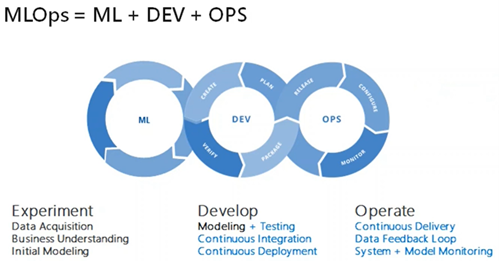
\includegraphics[width=7cm]{./img/img1.png}
\end{center}
\begin{center}
    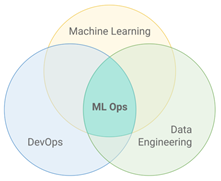
\includegraphics[width=7cm]{./img/img2.png}
\end{center}

\subsection{¿Por qué empezar a aplicar MLOps?}
\noindent En la actualidad, nos encontramos en un mundo orientado a datos, que está vinculado a la cantidad exponencialmente creciente de los mismos, recogidos digitalmente. Además, nos encontramos con la ascendente importancia de la Inteligencia Artificial y la Ciencia de Datos, que se deriva de esta tremenda cantidad de información generada.\\[0.1in]
Dependiendo de todos ellos, se pueden explotar de formas distintas, distinguiendo en capacidades (percepción, cognitivo y aprendizaje) y casos de uso (visión, audio, voz y lenguaje natural).

\subsection{¿Por qué MLOps?}
\noindent La mayoría de los científicos de datos no son programadores empedernidos. Pueden crear el modelo más eficaz para un problema de aprendizaje automático, pero no tienen las habilidades para empaquetar, probar, implementar o mantener este modelo en producción. Se necesita alguien con conocimiento de bases de datos, API REST y una colección de otras habilidades de TI para hacer eso. Aquí es donde entra en juego MLOps.\\[0.1in]
MLOps va más allá del desarrollo y diseño de modelos : también reúne la gestión de datos, el desarrollo automatizado de modelos, el reentrenamiento de modelos, la generación de código, el desarrollo continuo y la supervisión del modelo . Al llevar los principios de DevOps al aprendizaje automático, permite un ciclo de desarrollo más rápido, un mejor control de calidad y la capacidad de responder a los requisitos comerciales cambiantes.

\subsection{Beneficios de MLOps}
\begin{itemize}
    \item Modernización rápida mediante la colaboración con la gestión del ciclo de vida del aprendizaje automático
    \item Cree modelos y flujos de trabajo emulados
    \item Fácil uso de modelos de alta precisión
    \item Gestión eficaz de cada fase del ciclo de vida del aprendizaje automático
    \item También es útil para el sistema de gestión de recursos y su control.    
\end{itemize}

\subsection{Desafíos de MLOps}
\begin{itemize}
    \item Despliegue y automatización
    \item Reproducibilidad de modelos y predicciones.
    \item Diagnósticos
    \item Gobernanza y cumplimiento normativo
    \item Escalabilidad
    \item Colaboración
    \item Usos comerciales
    \item Seguimiento y gestión
\end{itemize}

\subsection{Qué tener en cuenta para usar MLOps}
\begin{itemize}
    \item \textbf{Calidad de los datos:} tener en cuenta de dónde vienen, calidad, si son fiables, etc.
    \item \textbf{Degradación de los modelos:} al cabo del tiempo van perdiendo calidad.
    \item \textbf{Localidad:} en el momento de la preparación se están entrenando los modelos con unos datos específicos basados en una geografía.
\end{itemize}

\subsection{Cómo es el proceso de MLOps}
\begin{itemize}
    \item \textbf{Diseño:} ajuste de requerimientos, establecer las necesidades que tienen los usuarios y qué queremos cubrir, exploración de los datos, experimentación.
    \item \textbf{Desarrollo del modelo:} desarrollo de un modelo funcional capacitado para pasar a producción.
    \item \textbf{Operaciones:} despliegue, automatización de entrenamientos, extracción de datos, etc.    
\end{itemize}

\subsection{¿Cuáles son los Principios de MLOps?}
\begin{itemize}
    \item \textbf{Automatización:} cuyas fases con proceso manual, ML pipeline y CI/CD pipeline.
    \item \textbf{Versionado:} basado en tres pilares, datos, modelo y código.
    \item \textbf{Testing:} base sobre la que va a funcionar todo el sistema.
    \item \textbf{Monitorización:} los puntos clave a tener en cuenta son que hay que estar atentos a que no haya cambios en dependencias, hay que asegurar los datos invariantes, el sesgo en predicciones, un modelo “rancio” que no es capaz de responder a la suficiente velocidad, modelo numéricamente estable y degradación del modelo.
    \item \textbf{Reproductividad:} de la ingeniería de características, del entrenamiento del modelo y del despliegue del modelo. Hay que tener cuidado con la recogida de datos, para poder reproducir los resultados.
    \item \textbf{Herramientas:} mlflow, DVC, Kubeflow, ONNX, TensorFlow Extended, Apache Airflow, Cookiecutter, Metaflow, jupyter, PyTorch o Psycaffold.    
\end{itemize}
\begin{center}
    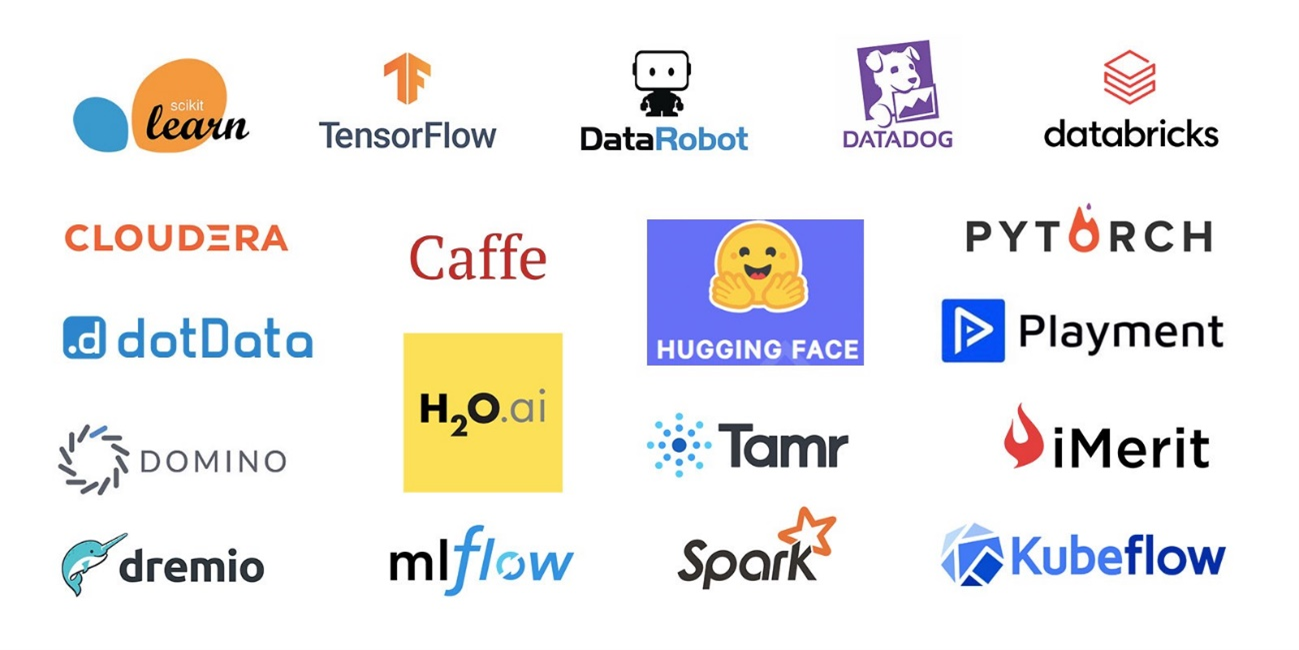
\includegraphics[width=7cm]{./img/img3.png}
\end{center}

%----------------------------------------------------------------------------------------
%	CONCLUSIONES
%----------------------------------------------------------------------------------------

\section{Conclusiones}
\noindent La inversión de tiempo en la configuración de MLOps puede ser considerable, pero los beneficios también son considerables, para una organización que se toma en serio el aprendizaje automático repetible en producción y la mantenibilidad a largo plazo. Las canalizaciones de ML automatizadas le permiten volver a capacitar y volver a implementar modelos, y la integración continua le permite garantizar que los procesos no se rompan y que los modelos continúen mejorando. El control de versiones de los datos y el código garantiza que pueda reproducir experimentos y rastrear los resultados de producción hasta los cambios originales.\\[0.1in]
A medida que el aprendizaje automático madura como campo, aparecen nuevos sistemas que facilitan la configuración de MLOps para su organización. En poco tiempo, MLOps probablemente se considerará tan común e importante como DevOps.

%----------------------------------------------------------------------------------------
%	RECOMENDACIONES
%----------------------------------------------------------------------------------------

\section{Recomendaciones}
\noindent MLOps, o DevOps para Machine Learning, permite a los equipos de ciencia de datos y TI colaborar y aumentar el ritmo del desarrollo y la implementación de modelos a través de la supervisión, validación y gobernanza de los modelos de Machine Learning.

%----------------------------------------------------------------------------------------
%	BIBLIOGRAFIA
%----------------------------------------------------------------------------------------

\begin{thebibliography}{99} 
    \bibitem{}
    Google Cloud. (s.f.). MLOps: canalizaciones de automatización y entrega continua en el aprendizaje automático. Recuperado de 
    \\\texttt{https://cutt.ly/lmsHAYQ}
    \bibitem{}
    KeepCoding. (2019). ¿Qué es MLOps? [Guía completa]. Recuperado de 
    \\\texttt{https://cutt.ly/lnod5w8}
    \bibitem{}
    Microsoft Azure. (2020). Operaciones de Machine Learning (MLOps). Recuperado de 
    \\\texttt{https://cutt.ly/wmsHH5j}
    \bibitem{}
    Alteryx. (s.f.). Operaciones de Machine Learning (MLOps). Recuperado de 
    \\\texttt{https://cutt.ly/cmsHVSc}
    \bibitem{}
    Towards Data Science. (2020). Get started with MLOps. Recuperado de 
    \\\texttt{https://cutt.ly/HmsH8XN}
\end{thebibliography}
%----------------------------------------------------------------------------------------
\end{document}